Our training pipeline combines two complementary data sources: the official
PAN-2026 competition corpus and a curated subset of the RAID benchmark.
Figure~\ref{fig:data_pipeline} provides a schematic overview of the data preparation
process.

\begin{figure}[t]
  \centering
  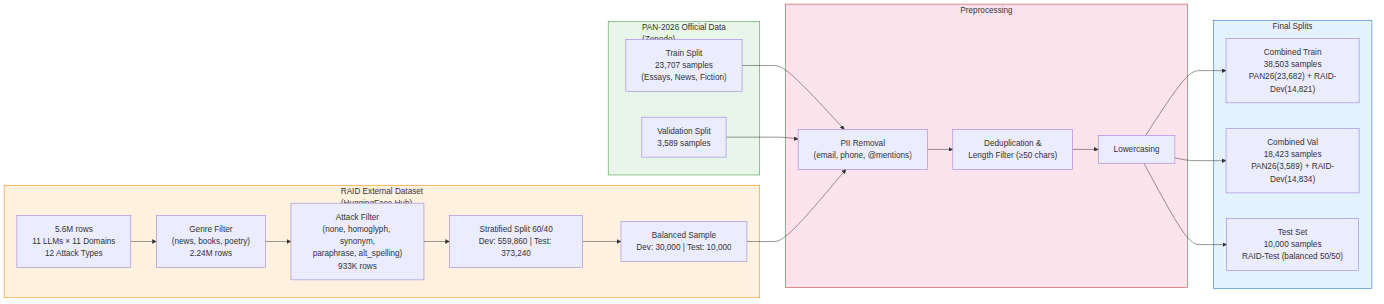
\includegraphics[width=\columnwidth]{images/data_pipeline.png}
  \caption{Overview of the data preparation pipeline. PAN-2026 official data and the
  RAID external dataset are preprocessed, filtered, and merged to form the final
  training, validation, and test splits.}
  \label{fig:data_pipeline}
\end{figure}

\subsection{PAN-2026 Dataset}

The official task corpus~\cite{bevendorff:2026overview} was downloaded from
Zenodo.\footnote{\url{https://zenodo.org/records/14962653}} It consists of newline-delimited
JSON files where each sample carries the fields \texttt{id}, \texttt{text}, \texttt{model},
\texttt{label} ($0 = \text{human}$, $1 = \text{AI}$), and \texttt{genre}.

The training split comprises 23,707 samples across three genres: \emph{essays} (diverse
expository writing), \emph{news} (articles from last year's PAN-2025 task with additional
GPT-4o samples), and \emph{fiction}. The validation split contains 3,589 samples drawn
from the same distribution.

\paragraph{Label distribution.} The training split is moderately imbalanced: 61.7\%
of samples are AI-authored and 38.3\% are human-authored. The genre distribution
is dominated by fiction (approximately 61.9\% of training samples), with essays
and news comprising the remainder.

\paragraph{AI generators.} The machine-authored samples in the training set were
produced by multiple models, including GPT-4o, Claude~3.5, Gemini~1.5~Pro, and
Llama~3-based models. Importantly, the LLMs were instructed to mimic a specific
human author's writing style, which substantially increases detection difficulty.

\subsection{RAID External Dataset}

To improve robustness to out-of-distribution generators and adversarial obfuscation,
we augment training with a subset of the RAID benchmark~\cite{dugan:2024}. RAID
contains approximately 5.6~million samples generated by 11~LLMs across 11~domains
and 12~adversarial attack types, making it the largest adversarially diverse AI-text
benchmark currently available.

\paragraph{Genre filtering.} We retain only three RAID domains that are semantically
aligned with the PAN-2026 genres: \emph{news} ($\leftrightarrow$ PAN news),
\emph{books} ($\leftrightarrow$ PAN fiction), and \emph{poetry} ($\leftrightarrow$ PAN essays).
After genre filtering, 2.24~million samples remain.

\paragraph{Attack filtering.} We retain five attack types that reflect the kinds
of obfuscation used in the PAN evaluation:

\begin{itemize}
  \item \texttt{none} — clean AI/human baseline samples;
  \item \texttt{homoglyph} — character-level Unicode substitution (used in the PAN test set);
  \item \texttt{synonym} — lexical paraphrase via synonym replacement;
  \item \texttt{paraphrase} — full sentence-level rewriting (hardest attack type);
  \item \texttt{alternative\_spelling} — region-based spelling variation.
\end{itemize}

After attack filtering, 933,100 samples remain.

\paragraph{Stratified split and sampling.} The filtered RAID set is split 60/40
(stratified by label) into a \emph{dev} pool (559,860 samples) and a held-out
\emph{test} set (373,240 samples). To keep training tractable on a single GPU and
to enforce a balanced signal, we draw a stratified subsample from the dev pool:
30,000 samples with exactly 50\% human and 50\% AI. The balanced RAID test subsample
(10,000 samples, 50/50) is used exclusively for out-of-domain evaluation. Attack
types are uniformly represented in the subsample (approximately 6,000 samples per
attack type in the dev sample).

\subsection{Data Preprocessing}

We apply a lightweight but consistent preprocessing pipeline to all splits:

\begin{enumerate}
  \item \textbf{PII removal}: email addresses, phone numbers, and Twitter/social-media
        user mentions (\texttt{@username}) are replaced with anonymous tokens
        (\texttt{[EMAIL]}, \texttt{[PHONE]}, \texttt{[USER]}).
  \item \textbf{Deduplication}: exact duplicate texts are removed.
  \item \textbf{Length filter}: texts shorter than 50 characters are discarded.
  \item \textbf{Lowercasing}: all text is converted to lower case to reduce sparsity
        in the stylometric feature space (tokenisation for the transformer is not
        affected, as the tokeniser handles casing internally).
\end{enumerate}

After preprocessing, the PAN-2026 training split reduces from 23,707 to 23,682 samples
(25 duplicates removed). All RAID samples pass the length filter as RAID texts are
generally long-form.

\subsection{Final Dataset Statistics}

Table~\ref{tab:dataset_stats} summarises the final dataset composition. The combined
training set contains 38,503 samples: 23,682 from PAN-2026 and 14,821 from the RAID dev
subsample (after the remaining RAID dev portion is allocated to validation). The validation
set (18,423 samples) combines the official PAN-2026 validation split with the remaining
RAID dev samples. The test set (10,000 samples, balanced 50/50) consists entirely of
the RAID test subsample and is used exclusively for cross-domain robustness evaluation.

\begin{table}[t]
\caption{Final dataset statistics for each split.}
\label{tab:dataset_stats}
\begin{tabular}{lrrrr}
\toprule
\textbf{Split} & \textbf{Total} & \textbf{Human} & \textbf{AI} & \textbf{Human \%} \\
\midrule
Train (PAN26 + RAID) & 38,503 & 16,449 & 22,054 & 42.7 \\
Val (PAN26 + RAID)   & 18,423 &  8,569 &  9,854 & 46.5 \\
Test (RAID only)     & 10,000 &  5,000 &  5,000 & 50.0 \\
\midrule
PAN26 Train          & 23,682 &  9,076 & 14,606 & 38.3 \\
PAN26 Val            &  3,589 &  1,277 &  2,312 & 35.6 \\
RAID Dev (subsample) & 30,000 & 15,000 & 15,000 & 50.0 \\
RAID Test (subsample)& 10,000 &  5,000 &  5,000 & 50.0 \\
\bottomrule
\end{tabular}
\end{table}
